\documentclass[twocolumn,showpacs,preprintnumbers,amsmath,amssymb,superscriptaddress,prb]{revtex4}

\usepackage{graphicx,amsmath,amsfonts,amssymb}% Include figure files and higher math
\usepackage{dcolumn}% Align table columns on decimal point
\usepackage{bm}% bold math
\usepackage{color}
\newcommand{\weirdsum}{\mbox{\textgoth{S}}}
\newcommand{\bgl}[1]{\mbox{\boldmath$#1$\unboldmath}}
\newcommand{\mbf}{\mathbf}

\begin{document}
\title{ Temperature Dependence of Ion Diffusion in Chromium Oxide $\textup{Cr}_2\textup{O}_3$ }

\author{Penghui Cao}
  \affiliation{Department of Nuclear Science and Engineering, Massachusetts Institute of Technology}
\author{Daniel Wells}
 \affiliation{Electric Power Research Institute (EPRI), Charlotte, NC 28262}
\author{Michael Short\footnote{Corresponding author: hereiam@mit.edu}}
 \affiliation{Department of Nuclear Science and Engineering, Massachusetts Institute of Technology}

\date{\today}% It is always \today, today, but any date may be explicitly specified

%%--------------------------------Abstract------------------------------
%%----------------------------------------------------------------------
\begin{abstract}

We apply molecular dynamics simulation to proce ion diffuion in chromium oxide $\textup{Cr}_2\textup{O}_3$. Point defects such as vacancy and interstital assisted diffusion mechanism is investigated, and their corresponding temperature dependent diffusion coefficients are also computed.Temperature-dependent diffusion anisotropy is observed in our simulation. At low temperature, ion diffusion is found to be strong anisotropic, which disappeard above 1800K. Migration energy barriers of point defects show the origin of this anisotropic diffusion and explain why it disappears at higher temperature. 

\end{abstract}

\maketitle

%%--------------------------------Section 1 ------------------------------
%%------------------------------------------------------------------------
\section{Introduction/Background}

\begin{itemize}
	\item $\textup{Cr}_2\textup{O}_3$ Oxides formed on steam generator alloy, ion diffusion is related to oxide growth and metal ion release. 
	\item experimental studies 
	\begin{enumerate}
		\item Sabioni et al. studied the role of oxygen and chromium ion diffusion on oxidation process and found chromium diffusivity is lower than the corresponding oxygen diffusivity. \cite{sabioni2012role}
		\item Lobnig et al. stidied the diffusion coefficients of Cr, Ni and Fe in $\textup{Cr}_2\textup{O}_3$ Oxides.\cite{lobnig1992diffusion} 
		\item Tsai \cite{tsai1996growth} probe growth mechanism of $\textup{Cr}_2\textup{O}_3$ Oxides by measuring oxygen and chromium diffusion. 
		\item Hoshino et al. measured Cr diffusion in plane and out of plane in single crystal of $\textup{Cr}_2\textup{O}_3$ and found diffusion along c axis is higher.  \cite{hoshino1983cation}
	\end{enumerate}
	\item MD studies 
	
    \begin{enumerate}
	   \item Ion diffusion \cite{vaari2015molecular} and surface properties \cite{sun2007molecular} have been studied by Vaari, Sun et al in chromium oxide by using MD. 
		 \item Ion diffusion by atomistic simulation. \cite{catlow1988atomistic} 
    \end{enumerate}
\end{itemize}

$\textup{Cr}_2\textup{O}_3$ oxide scales are usually formed on the surface of high chromium-bearing alloys and this chromium oxide layer plays an important role in protecting metallic alloys against corrosion. *Need to add something in LWRs, relate it to CRUD formation*. To understand oxidation and metal ion release processes, studying ions diffusion mechanism is desirable.  

\par The diffusion of chromium and oxygen ions in $\textup{Cr}_2\textup{O}_3$ has been investigated experimentally\cite{sabioni2012role,lobnig1992diffusion,tsai1996growth,hoshino1983cation} and computationally\cite{catlow1988atomistic,vaari2015molecular}. In Hoshino's experiment, self-diffusion of chromium ion has been found highly depends on diffusion direction. We found that ion diffusion in $\textup{Cr}_2\textup{O}_3$ has been little studied by using aomistic simulation. Just recently molecular dynamics simulation was applied to compute ion diffusivity due to Schottky type point defects. However, the directional anisotropic diffusion in $\textup{Cr}_2\textup{O}_3$ is still need to be uncovered.

The aim of this study is to understand poit defects assisted difussion mechanism in $\textup{Cr}_2\textup{O}_3$. We studied vacancy and inerstital diffusion of ion for a range of temperatures by means of MD simulation and found that temperature can affect  diffusion anisotropy. The on diffusion is found to be strong anisotropic at low temperatrue and the anisotropy disappears when temperate becomes higher. We then compute the activation energy barrier of ion migration by using Nudged Elastic Band (NEB) to interpret the origin of anisotropic diffusion.    


%%--------------------------------Section 2 ------------------------------
%%------------------------------------------------------------------------
\section{Computational Methods}
	
		In our present work, we modeled the interaction between ions by the combination of short range Buckingham potential and long range Coulombic potential. The potential for the interaction between ions $i$ and $j$ at a distance $r$ is defined as
		\begin{equation}
					U_{ij}(r) = A_{\text{ij}}e^{-r/\rho_{\text{ij}}} - \frac{C_{\text{ij}}}{r_{\text{ij}}} + \frac{q_\text{i}q_\text{j}}{4\pi\epsilon_0r_{\text{ij}}} 
		\end{equation}
		where the parameters $A$, $\rho$ and $C$ can be found in previous study \cite{---CITEpaper}. 
\par Like $\alpha - \textup{Al}_2\textup{O}_3$ and $\textup{Fe}_2\textup{O}_3$, $\textup{Cr}_2\textup{O}_3$ has the ctudum structure. **Add unit cell description and figure** Our simulations were carried out using a  $18\times18\times18$ hexagonal super cell system that contains 58320 atoms. We use periodic boundary conditions in all three directions. To study vacancy and interstitial assisted ion diffusion, we randomly delete or insert ionic atoms in the system. In our simulation model, vacancy or interstital has defects cencentraton of 0.0008. Before the diffusion coefficient calculation, the system is relaxted at zero pressure for 100 ps in the NPT (constant number of atoms, pressure and temperature) and another 100 ps run is performed in the NVT ensemble (constant number of atoms, volume and temperature). The Nose-Hoover thermostat is used in time intergration and the time step is set to be 1 fs. 
\par The ion diffusion was determinated measureing mean square displacement (MSD) of ions as a function of time at a range of temperatures. The MSD of ion is described by

\begin{equation}
	\big<\Delta{r}^2(t)\big> = \frac{1}{N} \sum_{i=1}^{N}{[\bold{r}_i(t+t_0) - \bold{r}_i(t_0)]^2}
\end{equation}
where N is total number of the ion in the system, $\bold{r}(t_0)$ is initial reference position at time $t_0$ and $\bold{r}(t)$ is position at time $t+t_0$. The diffusivity that relates MSD to the observe time $t$ is defined as  

\begin{equation}
D = \frac{\big<\Delta{r}^2(t)\big>}{2d\times t} 
\end{equation} 
where $d$ is dimensionality of the system. Then diffusivity of ion along $c$ axis, in $ab$ plane and in three dimensions can be calculated by $D_{c} = \big<\Delta{r}_c^2(t)\big>/2t$, $D_{ab} = \big<\Delta{r}_{ab}^2(t)\big>/4t$ , $D_{3} = \big<\Delta{r}_{abc}^2(t)\big>/6t$.  The diffusion coefficient $D$ is calculated by fitting the MSD as a function of time. All diffusion simuations are performed in NVT emsamble by extensive simulation time of 1 ns to ensure adequate statistical sampling.   

\begin{figure} 
	\centering
		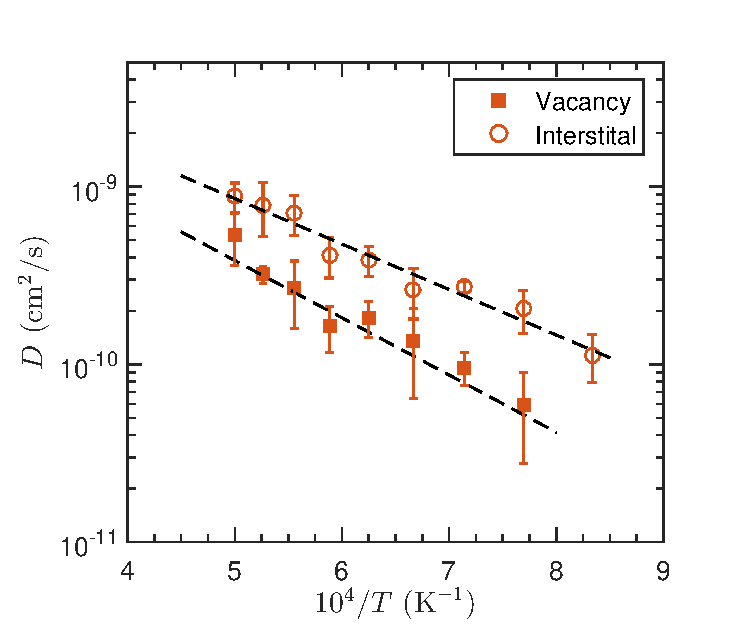
\includegraphics[scale=0.34]{./pics/Cr.eps}
		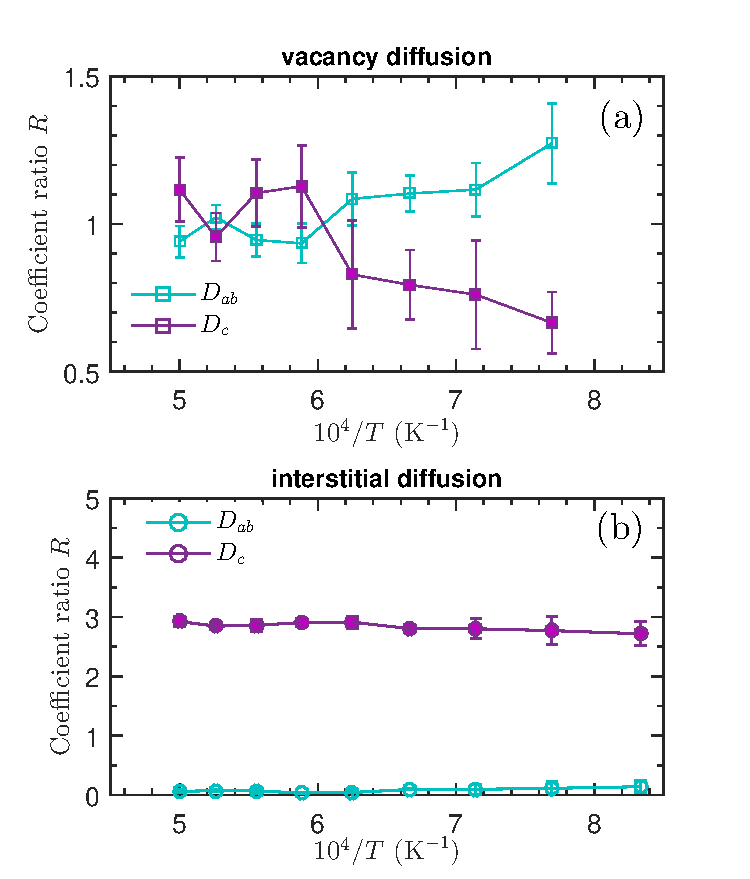
\includegraphics[scale=0.34]{./pics/Diffusion_ratio_Cr.eps}
	\caption{Chromium ion diffusivities in 3 dimensions, along $c$ axis and in $ab$ plane.  (left)Oxygen vacancy and interstitial diffusion coefficients as function of temperature, (right) (a)normalized chromium vacancy diffusivities $D_{ab}$ and $D_{c}$ in $ab$ plan and along $c$ axis, (b)normalized chromium interstital diffusivities in $ab$ plan and along $c$ axis}
	\label{fig1} 
\end{figure}

\begin{figure} 
	\centering
		\includegraphics[scale=0.34]{./pics/Oxygne.eps} 
		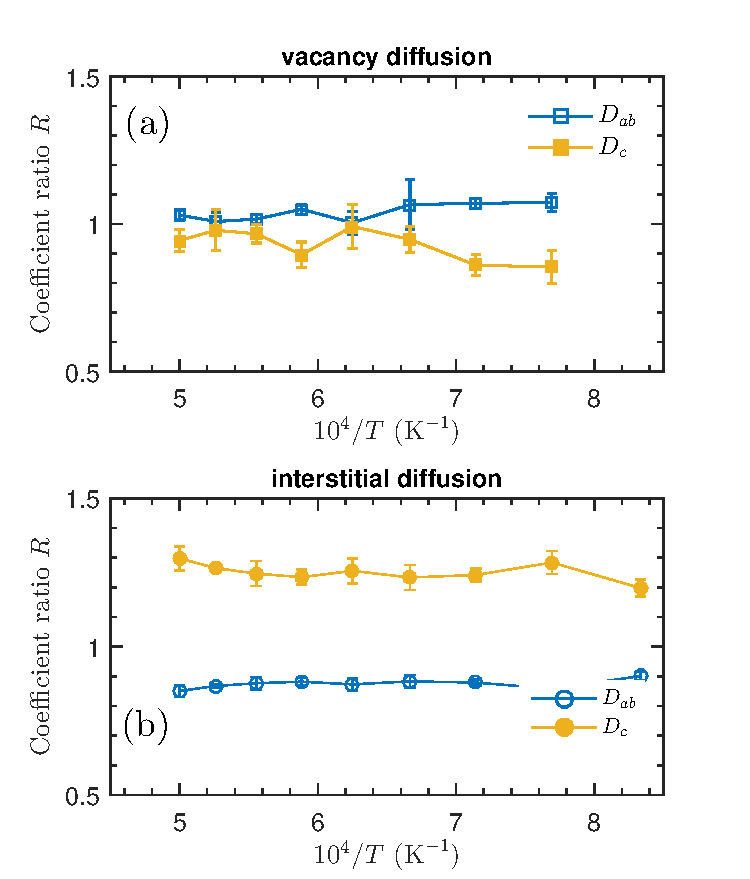
\includegraphics[scale=0.34]{./pics/Diffusion_ratio_Oxygen.eps}
	\caption{Oxygen ion diffusivities in 3 dimensions, along $c$ axis and in $ab$ plane.  (left)oxygen vacancy and interstitial diffusion coefficients as function of temperature, (right) (a)normalized oxygen vacancy diffusivities $D_{ab}$ and $D_{c}$ in $ab$ plan and along $c$ axis, (b)normalized oxygen interstital diffusivities in $ab$ plan and along $c$ axis} 
	\label{fig2} 
\end{figure}


%%--------------------------------Section 3 ------------------------------
%%------------------------------------------------------------------------
\section{Resultss}
\subsection{Temperature-dependent ion diffusivities}

Our simulation are performed at temperature ranging from 1200 K to 2000 K ad the diffusion coefficients determined at vacancy defect interstital defect are shown in Fig. \ref{fig1} and \ref{fig2}.   

\subsection{Point defects migration pathways}
\begin{figure} 
	\centering
		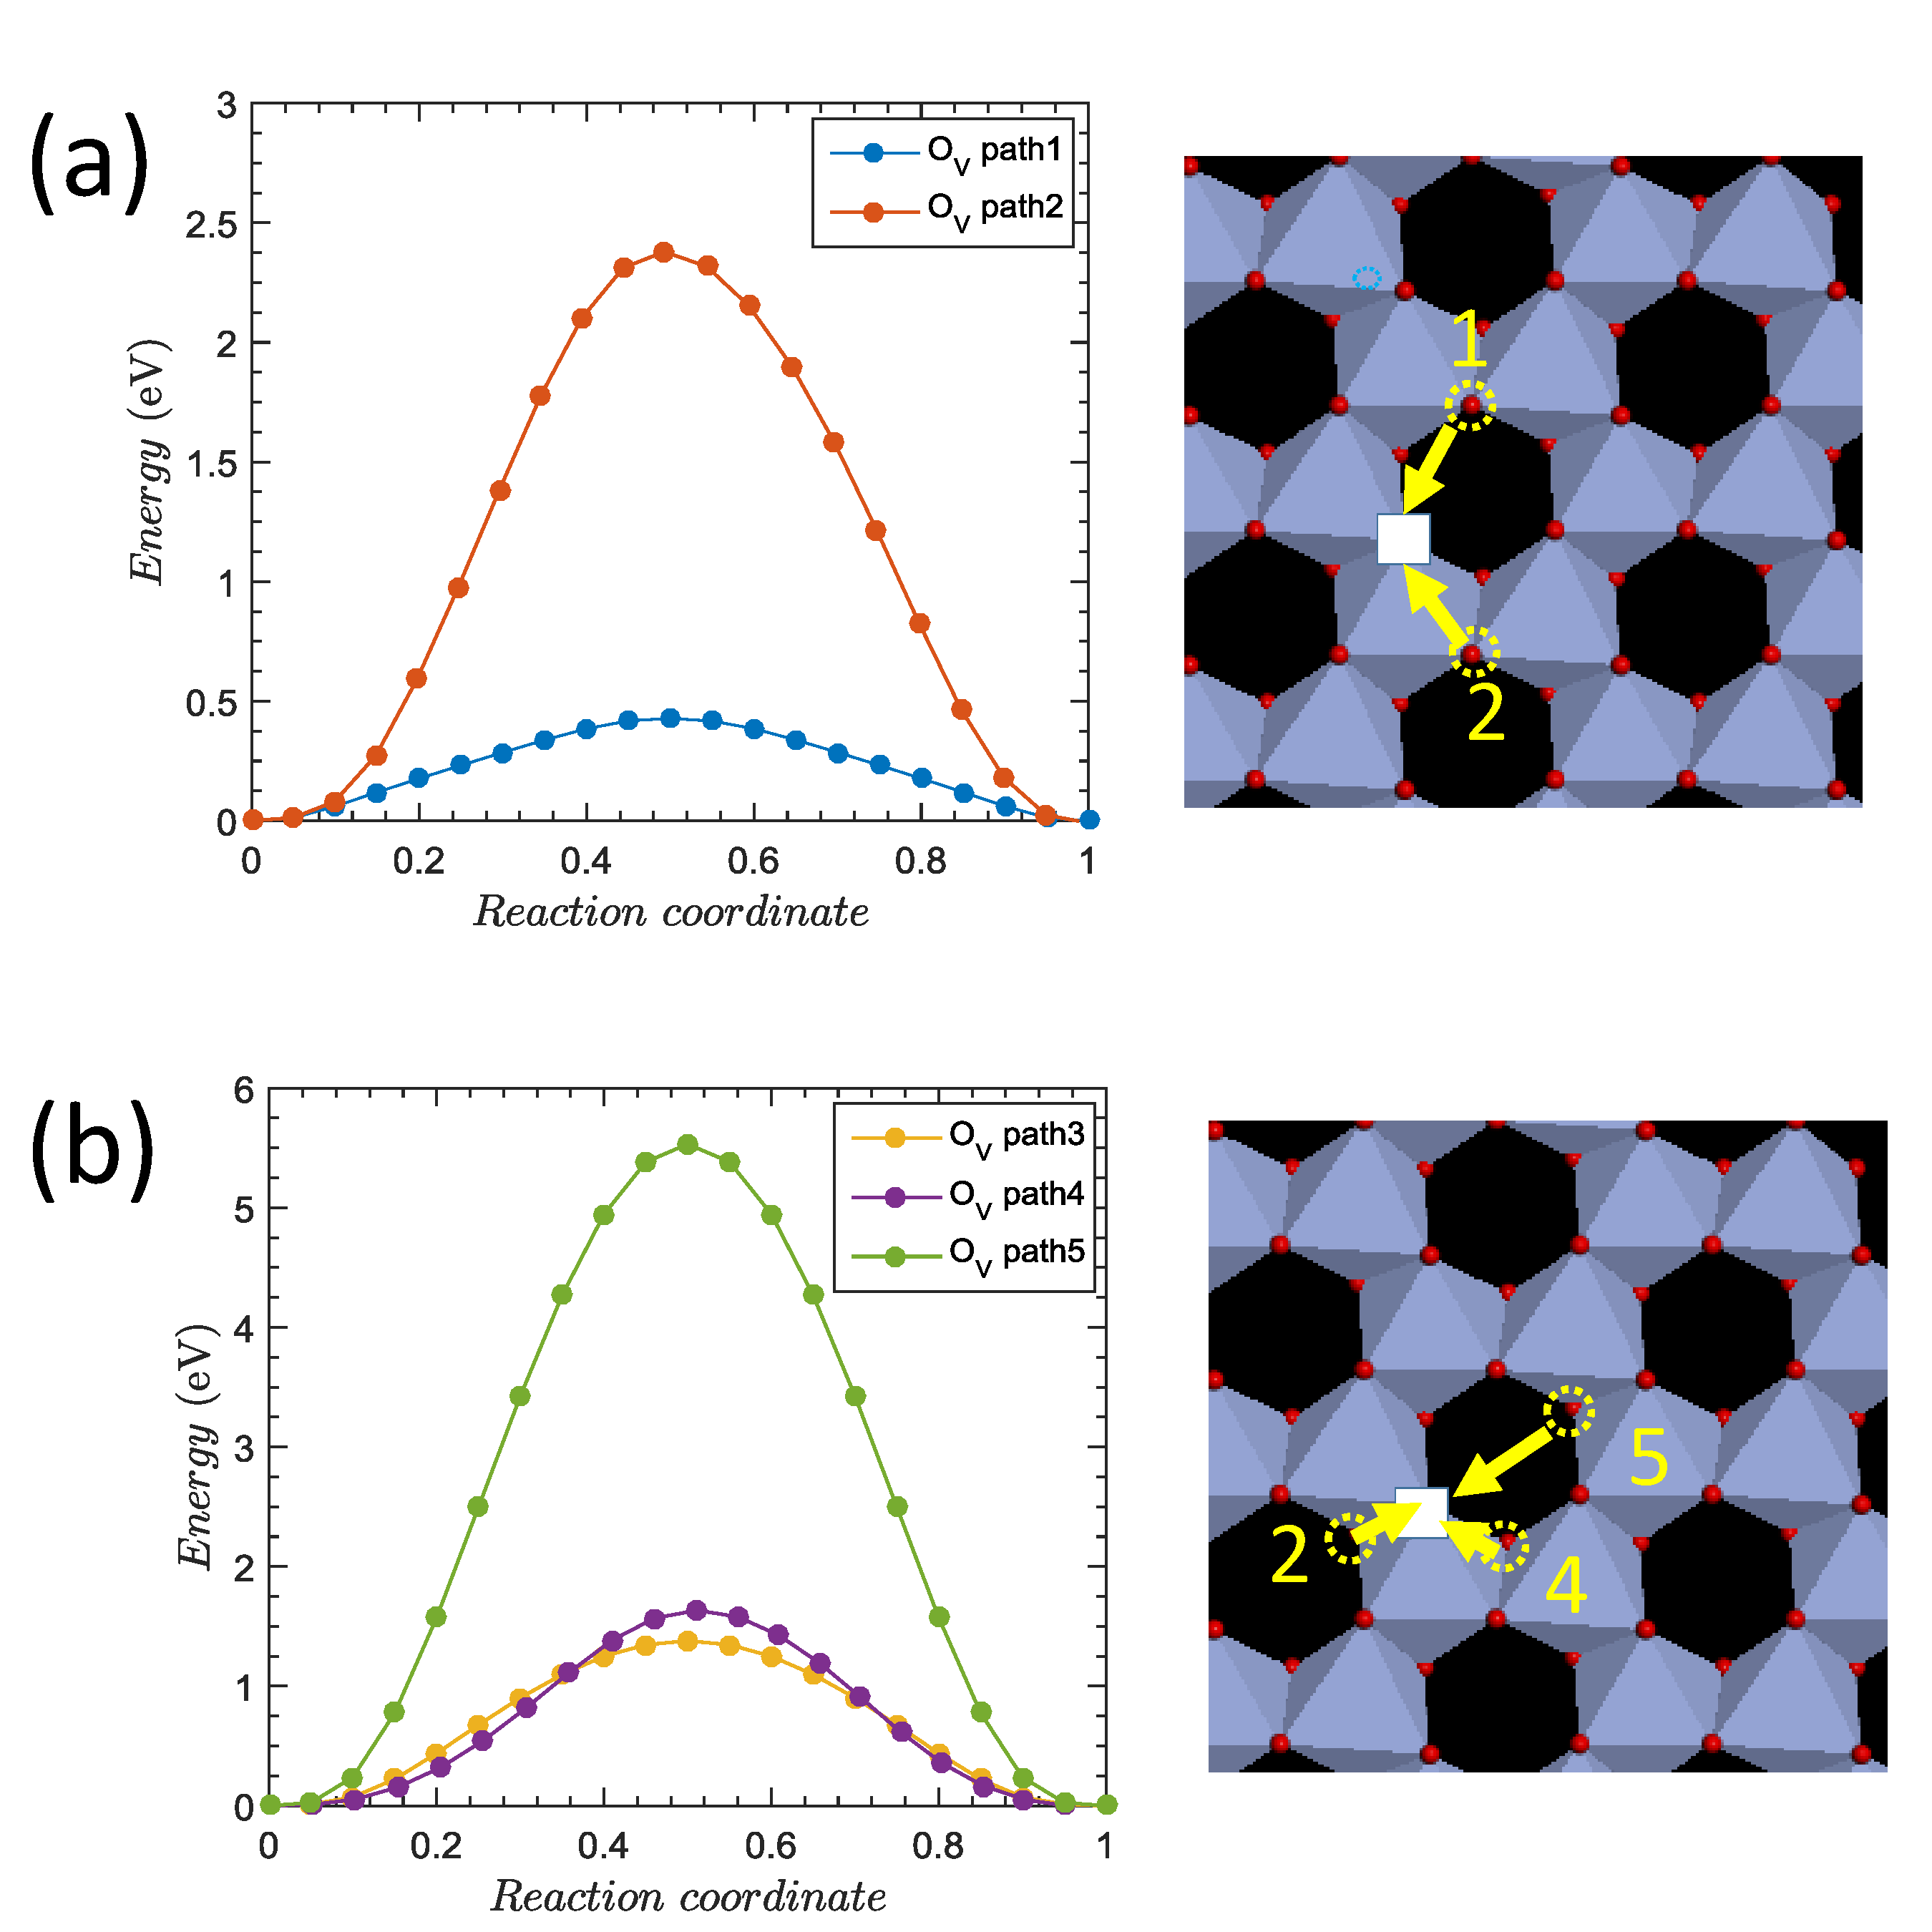
\includegraphics[scale=0.15]{./pics/Oxygen_vacancy_path.pdf}
	\caption{Oxygen vacancy migration pathways. (a) paths in $ab$ plane, (b) out of plane paths }
	\label{fig5} 
\end{figure}
\begin{figure} 
	\centering
		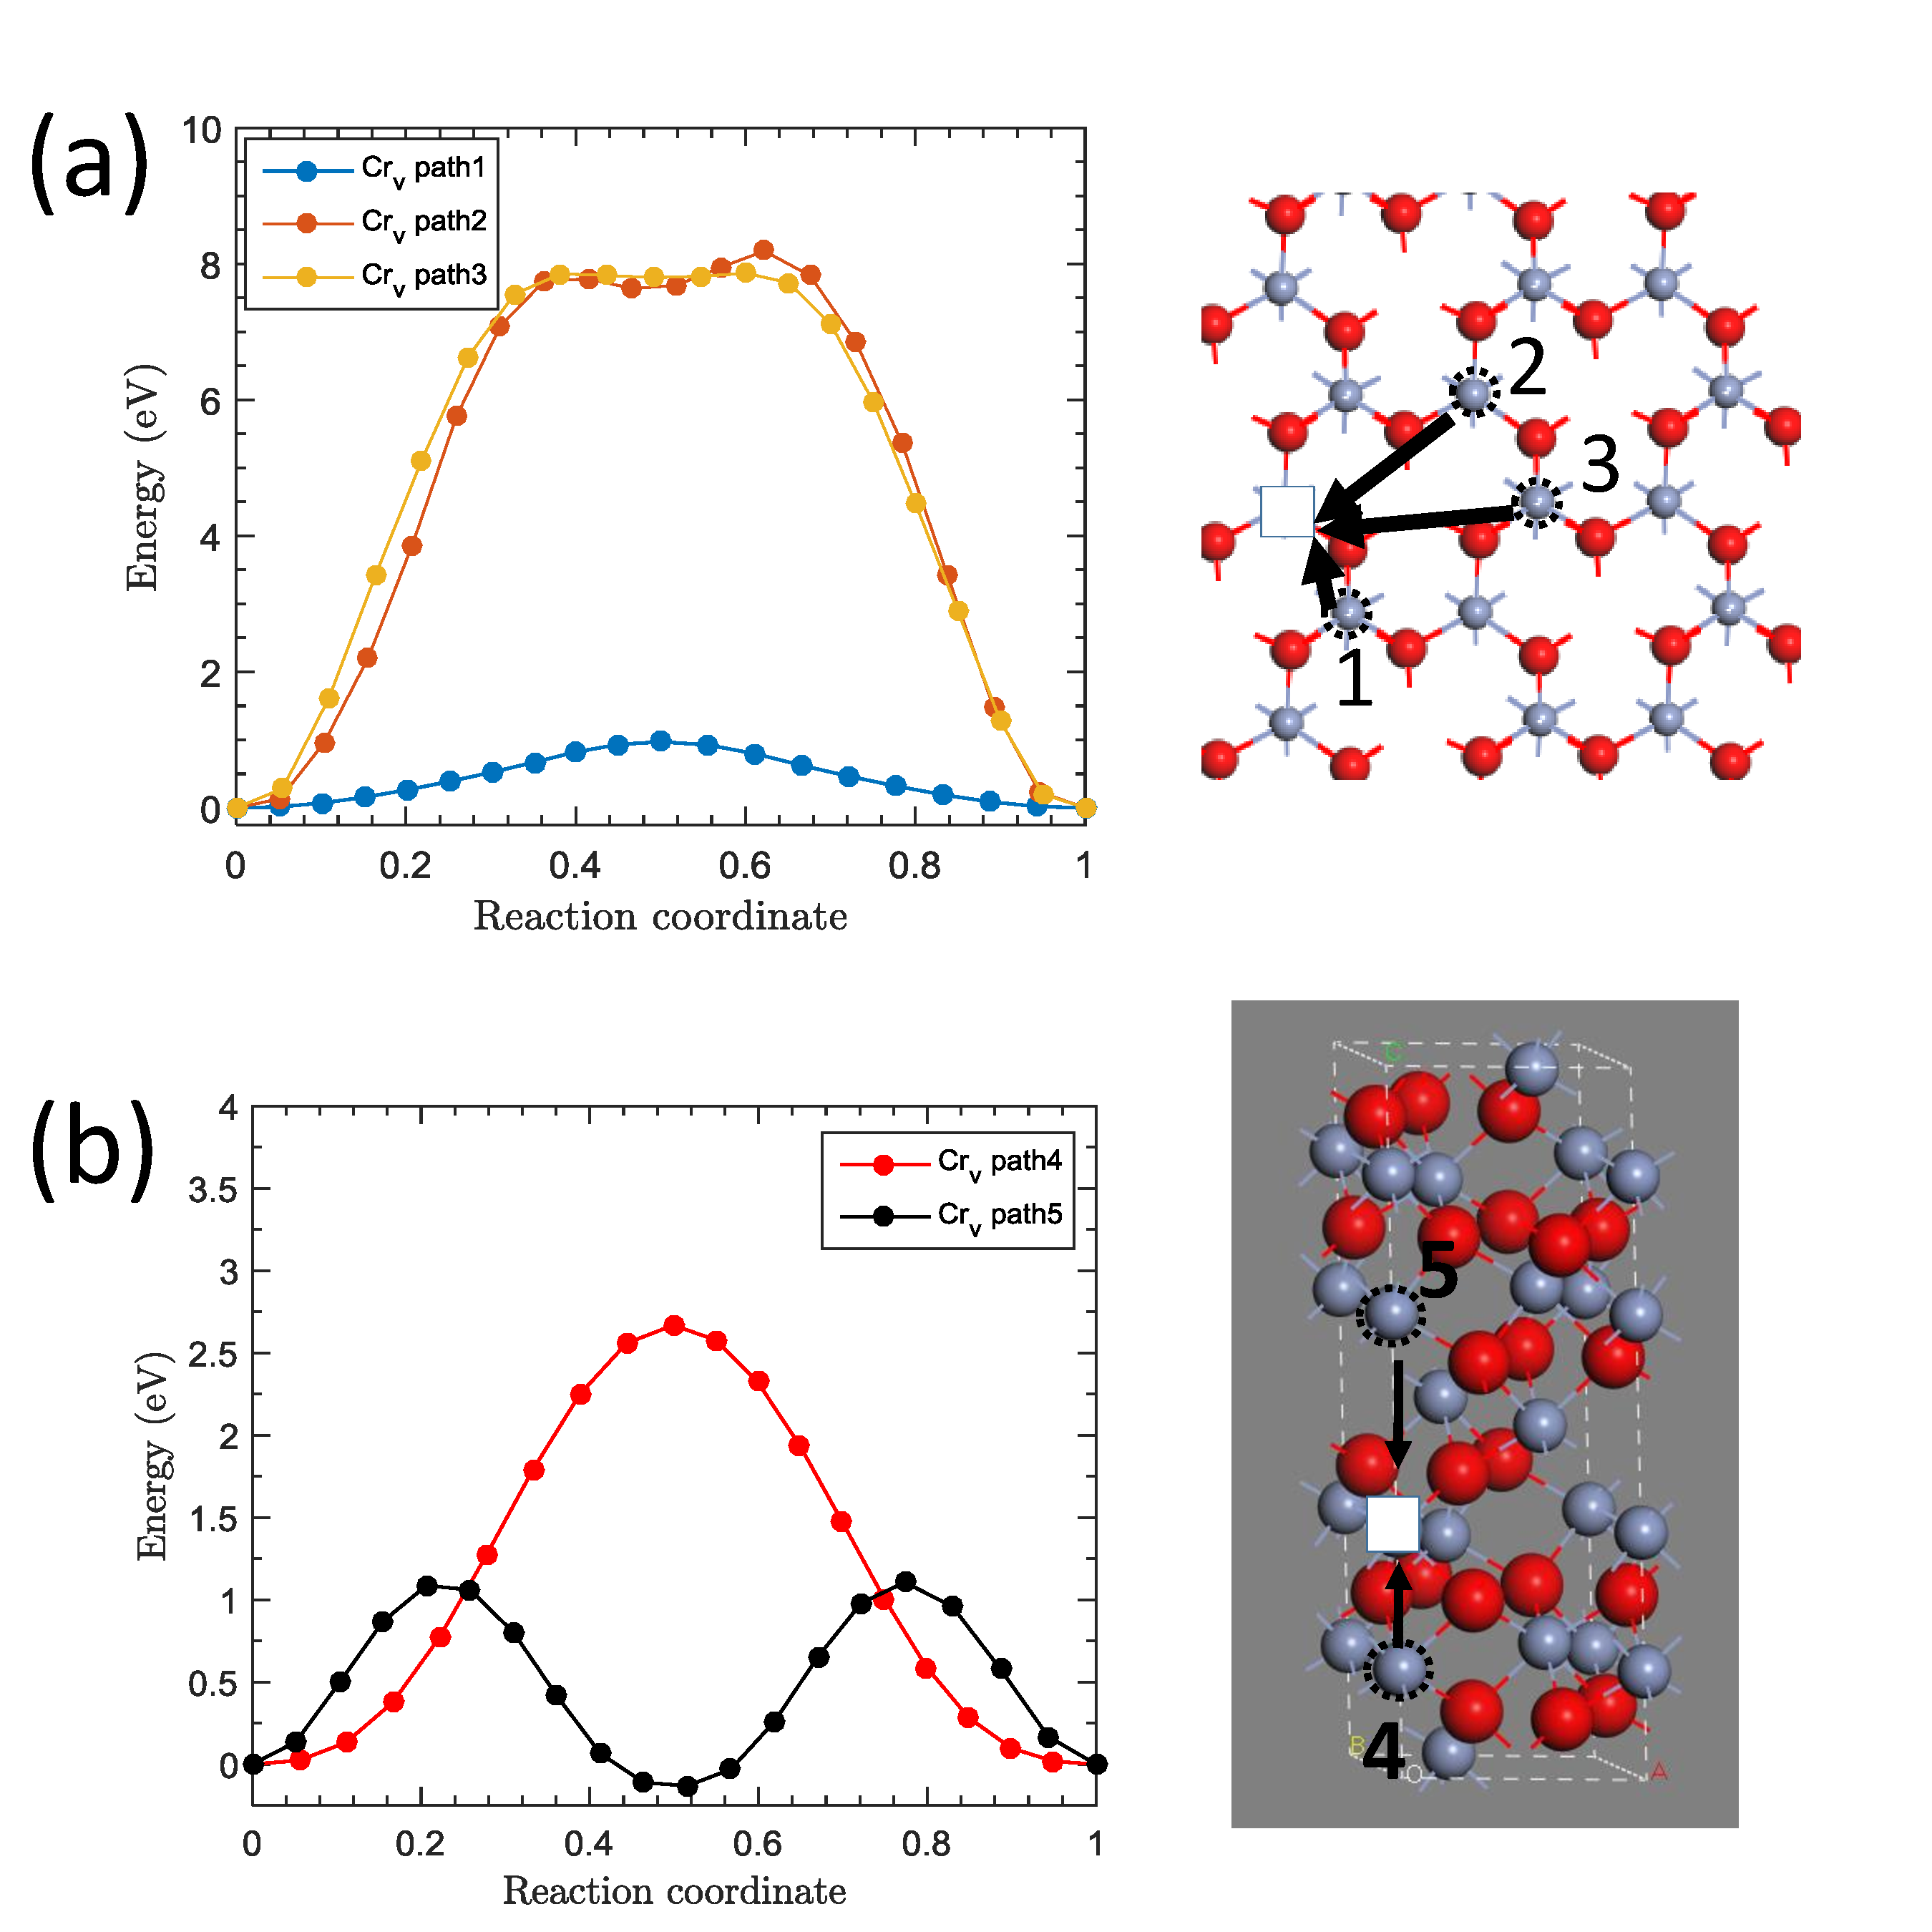
\includegraphics[scale=0.15]{./pics/Cr_vacancy_path.pdf}
	\caption{Chromium vacancy migration pathways. (a) paths in $ab$ plane, (b) out of plane paths }
	\label{fig6} 
\end{figure}

\begin{figure} 
	\centering
		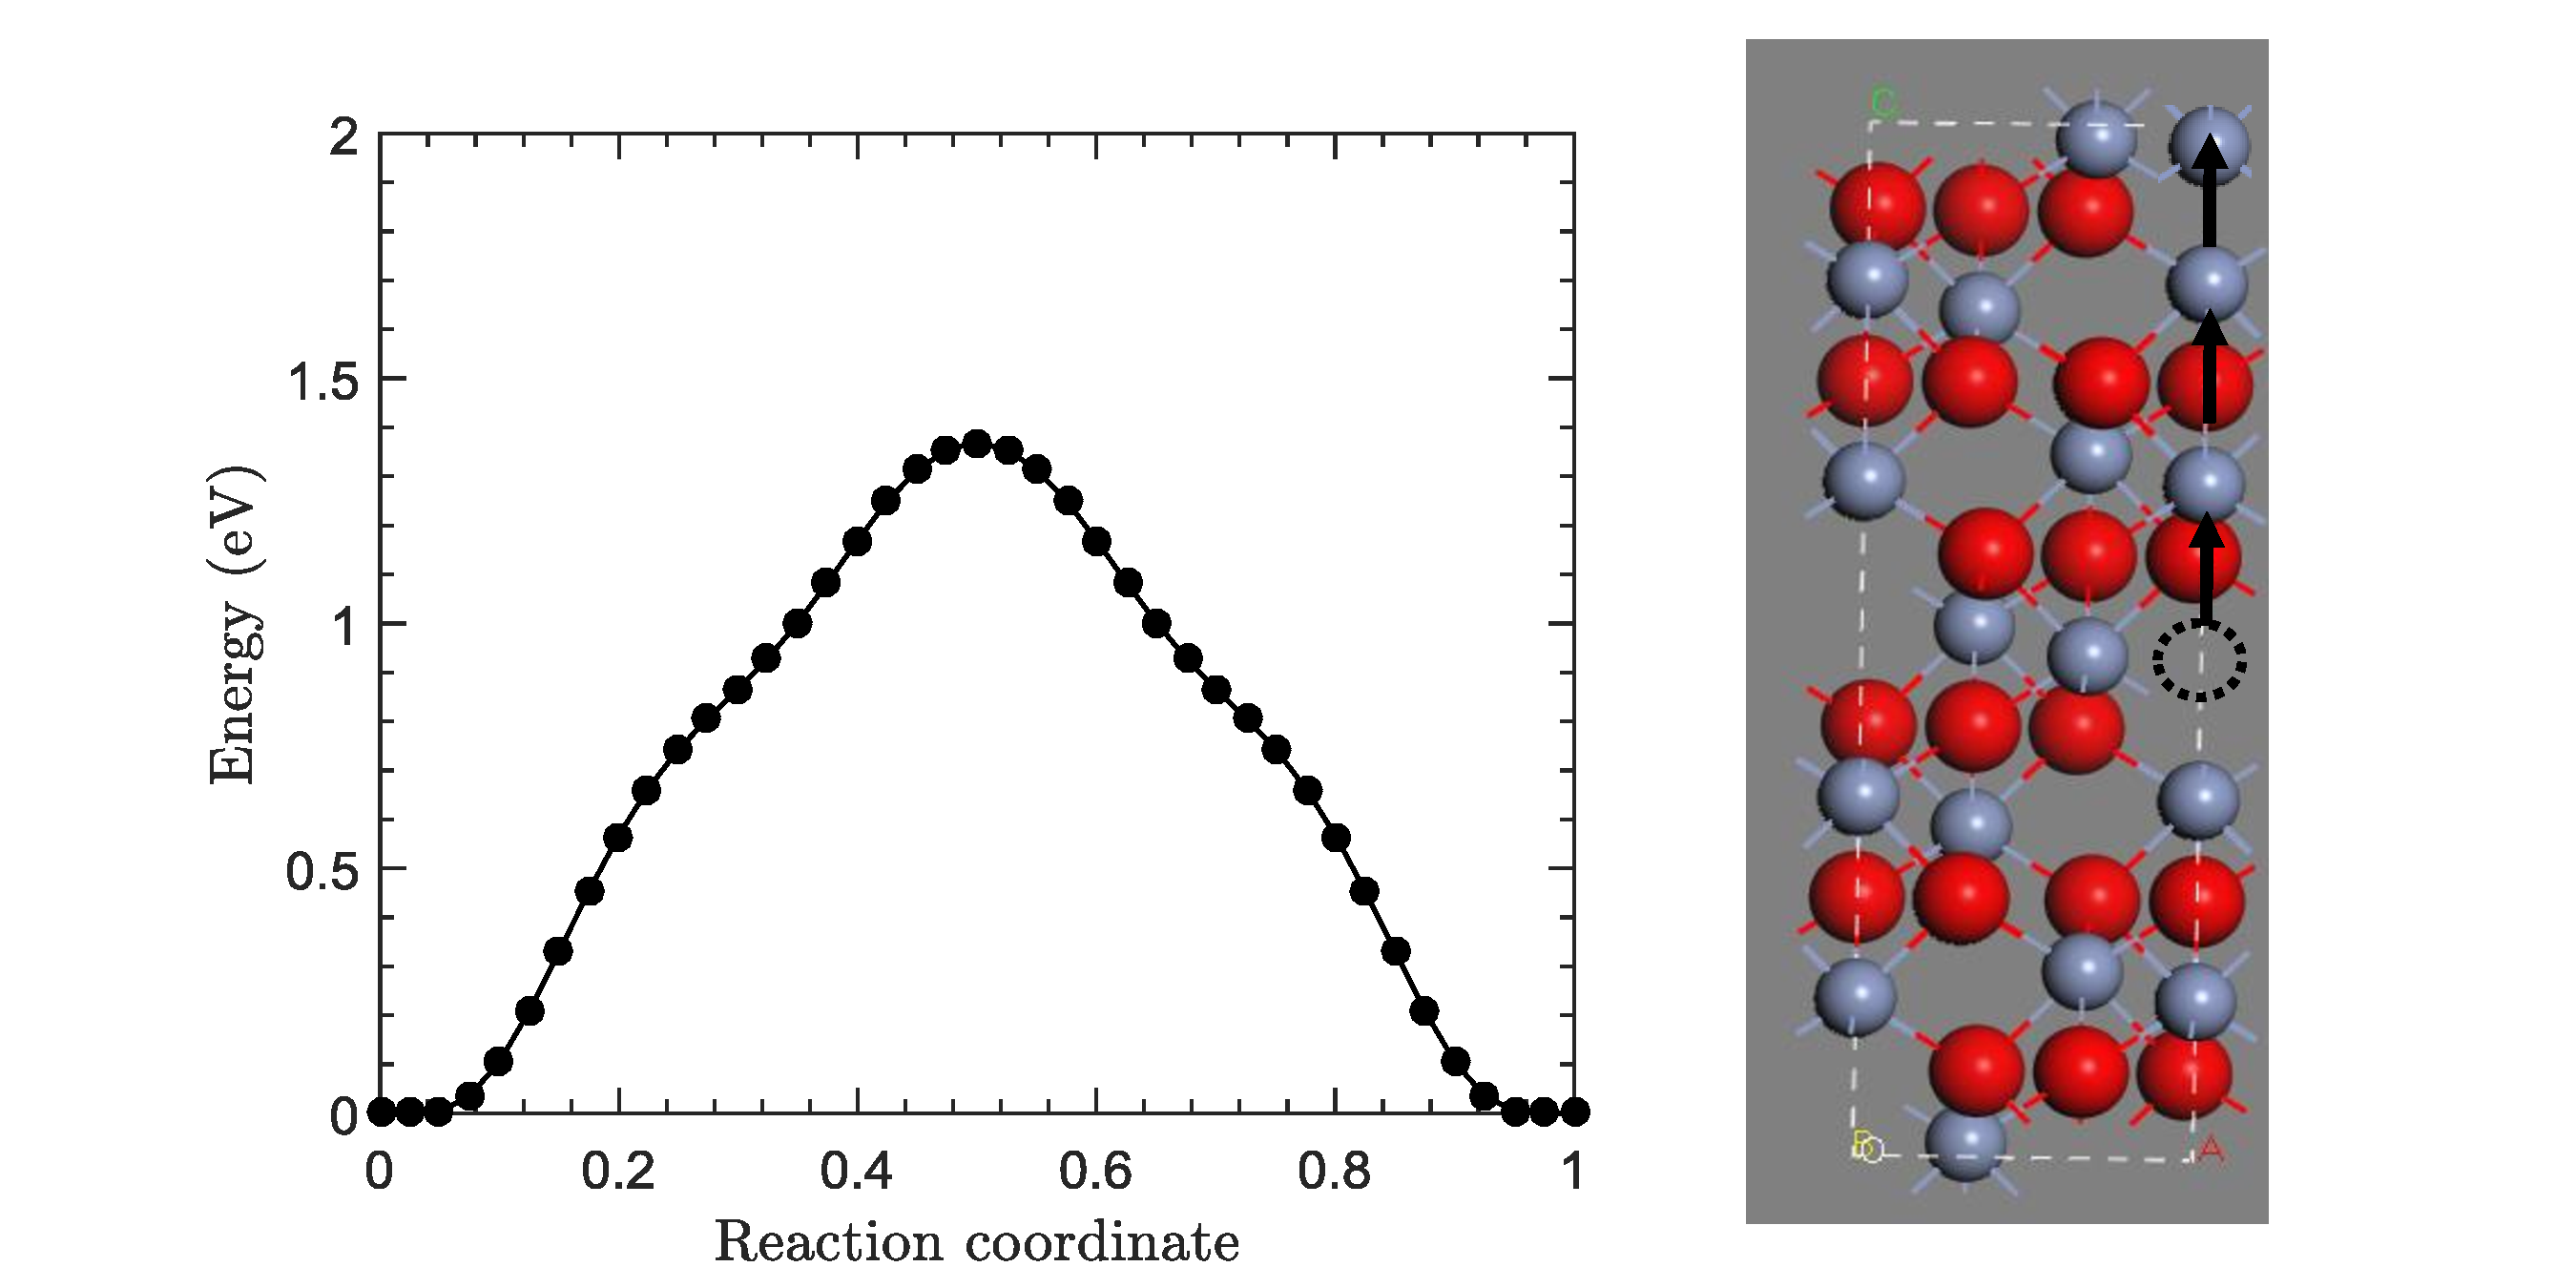
\includegraphics[scale=0.15]{./pics/Cr_inter_path.pdf}
	\caption{Chromium interstitial migration pathway}
	\label{fig7} 
\end{figure}


\begin{itemize}
	\item Oxygen vacancy migration pathways, Fig. \ref{fig5} 
	\item Chromium vacancy migration pathways, Fig. \ref{fig6}  
	\item Chromium interstitial migration pathway, Fig. \ref{fig7}   
\end{itemize}



%%--------------------------------Section 4 ------------------------------
%%------------------------------------------------------------------------
\section{Discussion}

Our diffusivity results are obtained at a defects concentration of 0.0008. However, we note that the diffusion coefficients of ion depends both on the concentration of defects and the mobility, as shown by
\begin{equation}
D(T) = \alpha a^2 C \omega = \alpha a^2 C fe^{-E_m/k_{B}T} 
\end{equation}
where $\omega$ is successful jump frequency, $f_{Debye}$ is tril frequency, $E_m$ is defect migration energy, $k_B$ is the Boltzmann constant, $T$ is system temperature, $\alpha$ is constant, $a$ is jump distance and $C_{defect}$ is concentration of defect. We also note that cencentrtion $C$ can be defind as 

\begin{equation}
C = e^{-E_f/k_BT}
\end{equation} 
where $E_f$ is defect formation energy. The above diffusivity equation there can be written as 
\begin{equation}
D(T)  = \alpha a^2 f e^{-E_f/k_BT}e^{-E_m/k_{B}T} 
\end{equation}. 
 

%%--------------------------------Figures------------------------------
%%------------------------------------------------------------------------


\bibliography{bib_diffusion}

\end{document}
